\documentclass[12pt]{article}
\usepackage[utf8]{inputenc}
\usepackage[mongolian]{babel}
\usepackage{graphicx}
\begin{document}
		\title{Системийн танилцуулга}
Багаар хөгжүүлж буй манай систем болох Eschool  нь оюутан, эцэг эх, багш гэсэн үндсэн гурван  хэрэглэгчтэй бөгөөд багш дүн, ирцийн мэдээлэл, хуваарь болон бүсад хэргэгтэй материалуудыг оруулах сурагч нь мөн багшийн оруулсан мэдээллүүдийг харах, гэрийн даалгавар бие даалтуудаа явуулах зэрэг үйлдлүүдийг хийх боломжтой. Эцэг эх нь уг системийн хэрэглэгч болохын тулд өөрийн хүүхдийнхээ Account-руу хүсэлт илгээх ба энэ хүсэлтийг оюутан баталгаажуулснаар эрх идэвхжиж эцэг эх гэсэн status-аар системийн хэрэглэгчээр бүртгэгднэ. Эцэг эх нь Eschool-ийн хэрэглэгч болсоноор өөрийн хүүхдийн дүнг, ирц, явц зэрэг мэдээллүүдийг харах, өөрийг Profile-аа шинэчлэх зэрэг эрхтэйгээр оролцно.
\section{ Функциональ шаардлага }
\begin{itemize} 
	\item Нэвтрэх
	\item Profile бөглөх
	\item Системийн хэрэглэгчээр бүртгүүлэх хүсэлт илгээх(өөрийн хүүхэдрүү)
	\item Хүүхдийнхээ үзэж буй хичээлүүдийн дүнг харах
	\item Ирцийн мэдээлэл харах
\end{itemize}
\subsection{Use Case диаграм}
\begin{figure}
	\caption{UseCase.}
	\label{fig:usecase}
	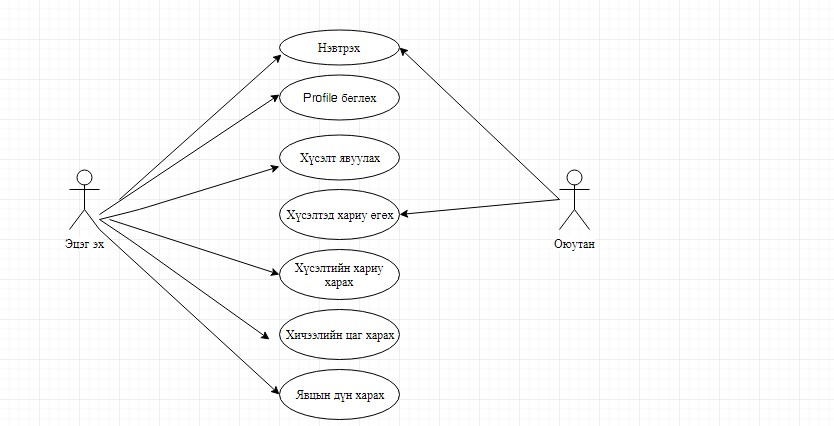
\includegraphics[width=\linewidth]{usecase.jpg}
\end{figure}
\begin{figure}
	\caption{BPMN.}
	\label{fig:bpmn1}
	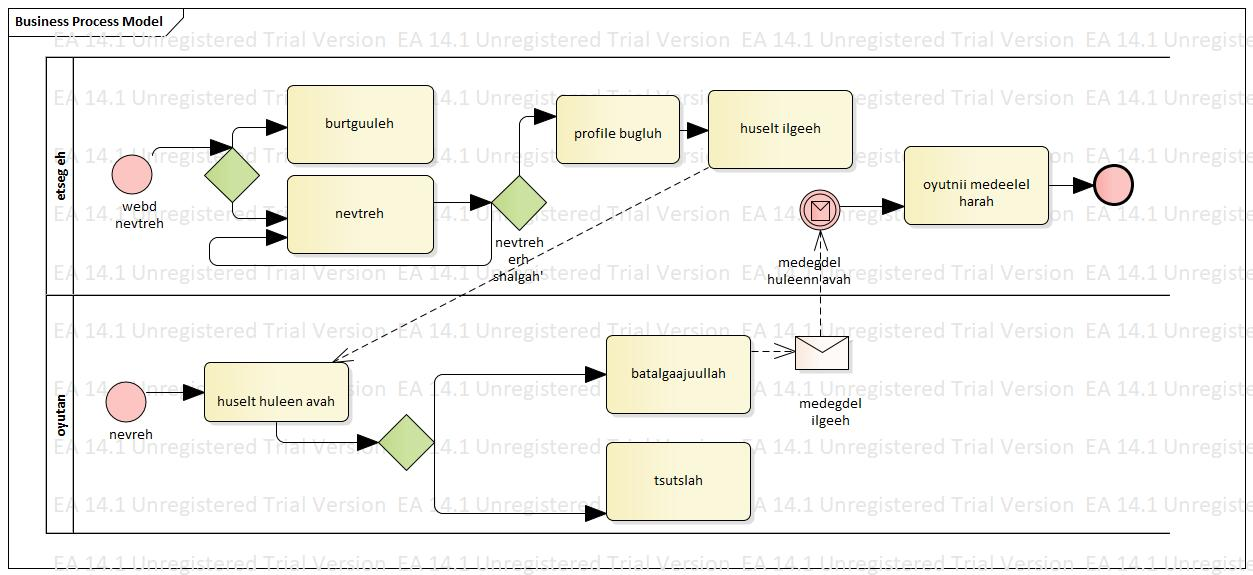
\includegraphics[width=\linewidth]{bpmn.jpg}
\end{figure}
\begin{figure}
	\caption{Activity1.}
	\label{fig:a1}
	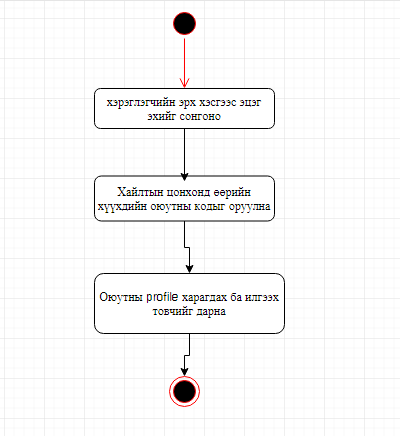
\includegraphics[width=\linewidth]{A1.png}
\end{figure}
\begin{figure}
	\caption{Activity2.}
	\label{fig:a2}
	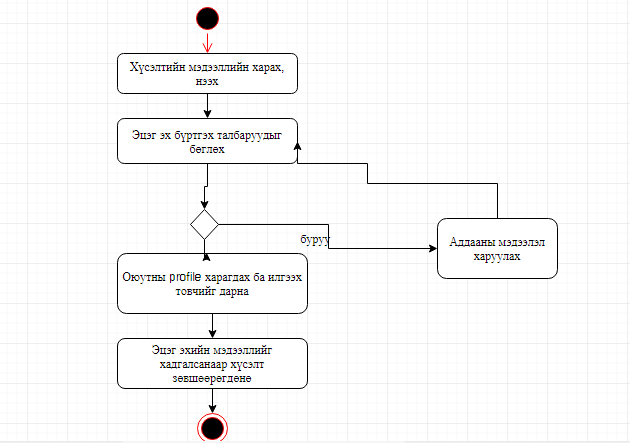
\includegraphics[width=\linewidth]{A2.png}
\end{figure}
\begin{figure}
	\caption{Activity3.}
	\label{fig:a3}
	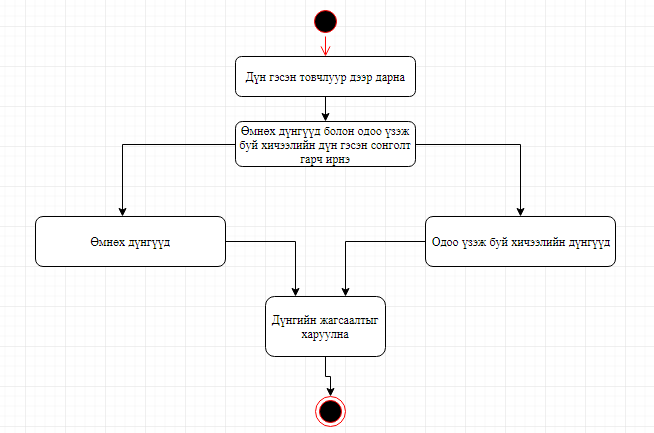
\includegraphics[width=\linewidth]{A3.png}
\end{figure}
\begin{figure}
		\caption{Activity4.}
	\label{fig:a4}
	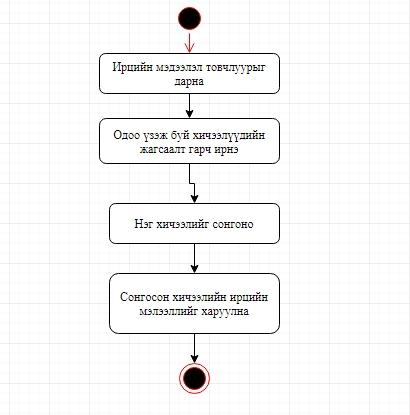
\includegraphics[width=\linewidth]{A4.png}
\end{figure}
\begin{figure}
		\caption{Sequence1.}
	\label{fig:s1}
	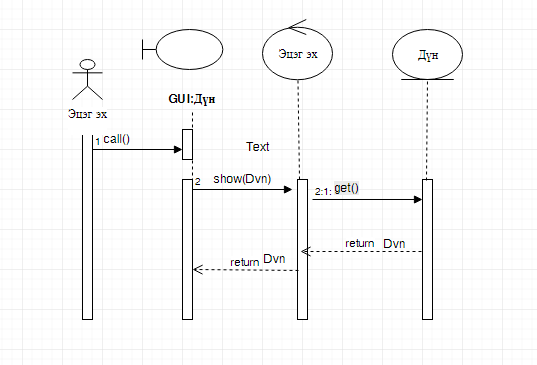
\includegraphics[width=\linewidth]{S1.png}
\end{figure}
\begin{figure}
			\caption{Sequence2.}
	\label{fig:s2}
	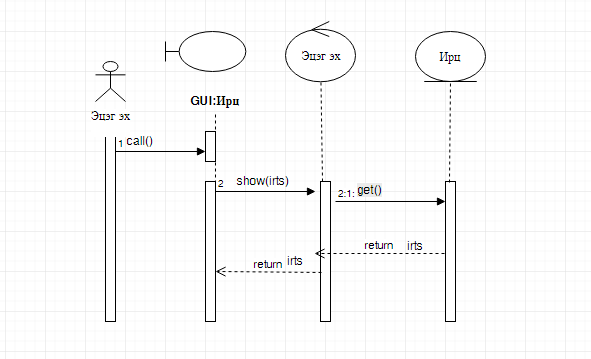
\includegraphics[width=\linewidth]{S2.png}
\end{figure}
\begin{figure}	
			\caption{ERD.}
	\label{fig:erd}
	\includegraphics[width=\linewidth]{ParentERD.jpg}
\end{figure}
\begin{figure}	
			\caption{Class.}
	\label{fig:class}
	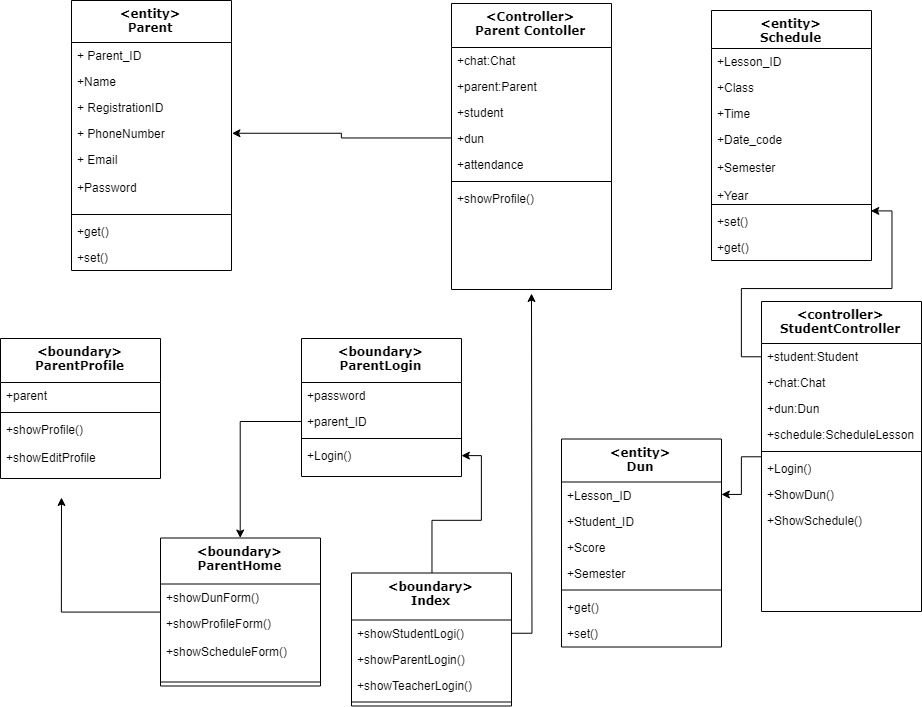
\includegraphics[width=\linewidth]{class.jpg}
\end{figure}	
\end{document}
